	\section{Use Case Diagram}
\begin{figure}[h]
	\centering
	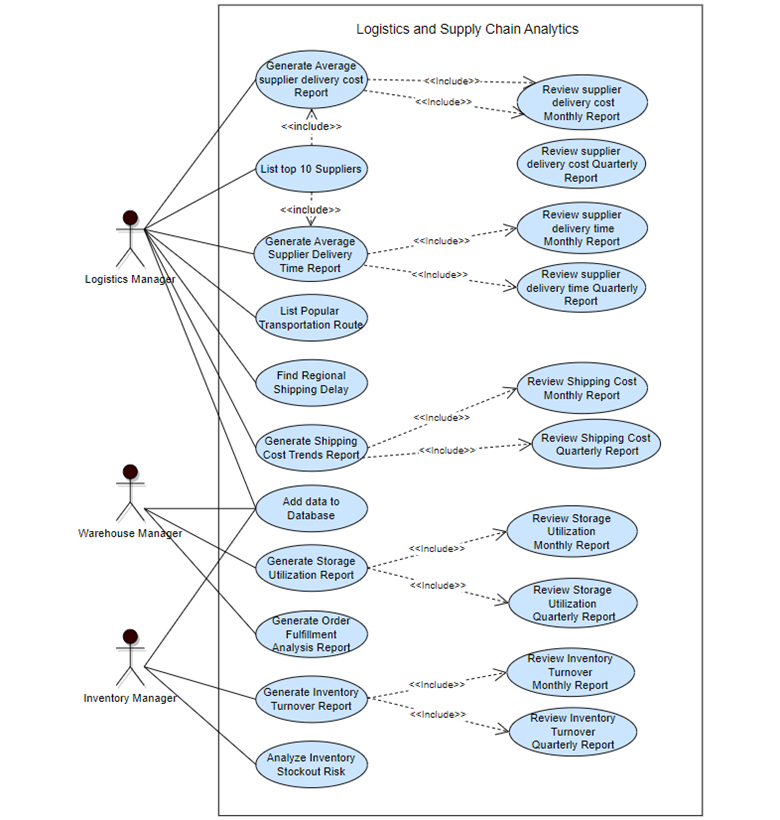
\includegraphics[width=1\textwidth]{UML.png} 
	\caption{Use Case Model}
	\label{fig:Use Case Model}
\end{figure}

\section{Use Cases}
\textbf{Actor Definitions:}
\begin{itemize}
	\item \textbf{Logistics Managers}: These users oversee transportation, shipping, and supplier operations and relation.
	\item \textbf{Warehouse Managers}: They manage warehouse operations, including storage space utilization and order fulfillment.
	\item \textbf{Inventory Managers}: These users are responsible for inventory management based on shipment and supplier information and turnover rate analysis.
\end{itemize}
\begin{center}
	\begin{tabularx}{\textwidth}{|l|X|}
		\hline
		System & METRICSTICS \\
		\hline
		Identifier & UC-1 \\
		\hline
		Author(s) & \begin{itemize}[left=0pt]
			\item Author Name: Sharanyu Pillai
			\item Author Email: sharanyu@hotmail.com
		\end{itemize} \\
		\hline
		Version & 1.0 \\
		\hline
		Priority & Medium \\
		\hline
		Name & Calculating Average supplier delivery cost for the stock procured \\
		\hline
		Pre-Condition(s) &  \begin{itemize}[left=0pt]
			\item User has a valid account on the system.
			\item Supply stock data is available in the system.
		\end{itemize} \\
		\hline
		Post-Condition(s) & \begin{itemize}[left=0pt]
			\item Average monthly and quarterly delivery cost report is generated.
		\end{itemize} \\
		\hline
		Trigger & Logistics Manager initiates the analysis. \\
		\hline
		Normal Flow & \begin{enumerate}[left=0pt]
			\item Logistics Manager logs into the system.
			\item Logistics Manager  selects the supply delivery cost analysis option.
			\item Logistics Manager  inputs new supply delivery cost data.
			\item System generates an analysis report.
		\end{enumerate} \\
		\hline
		Exceptional Flow & None \\
		\hline
		Related Actor(s) & Logistics Manager \\
		\hline
		Related Use Case(s) & None \\
		\hline
		Description & Logistics Manager averages shipping cost for the supply obtained monthly and quarterly to make improvements and reduce expenses in the future. \\
		\hline
	\end{tabularx}
\end{center}

\begin{center}
	\begin{tabularx}{\textwidth}{|l|X|}
		\hline
		System & METRICSTICS \\
		\hline
		Identifier & UC-2 \\
		\hline
		Author(s) & \begin{itemize}[left=0pt]
			\item Author Name: Sharanyu Pillai
			\item Author Email: sharanyu@hotmail.com
		\end{itemize} \\
		\hline
		Version & 1.0 \\
		\hline
		Priority & High \\
		\hline
		Name & Supplier Delivery Time Trends \\
		\hline
		Pre-Condition(s) &  \begin{itemize}[left=0pt]
			\item Valid user account in the system.
			\item Availability of supplier delivery time data.
		\end{itemize} \\
		\hline
		Post-Condition(s) & \begin{itemize}[left=0pt]
			\item Supplier delivery time trend report generated.
		\end{itemize} \\
		\hline
		Trigger & Logistics Manager initiates analysis. \\
		\hline
		Normal Flow & \begin{enumerate}[left=0pt]
			\item Logistics Manager logs in.
			\item Selects supplier delivery time trend analysis.
			\item Inputs delivery time data.
			\item System generates supplier delivery time trend.
		\end{enumerate} \\
		\hline
		Exceptional Flow & None \\
		\hline
		Related Actor(s) & Logistics Managers \\
		\hline
		Related Use Case(s) & None \\
		\hline
		Description & Logistics Managers analyze supplier delivery time trends to identify months and quarters with significant changes. \\
		\hline
	\end{tabularx}
\end{center}

\begin{center}
	\begin{tabularx}{\textwidth}{|l|X|}
		\hline
		System & METRICSTICS \\
		\hline
		Identifier & UC-3 \\
		\hline
		Author(s) & \begin{itemize}[left=0pt]
			\item Author Name: Wei Qi
			\item Author Email: qiwei12181@163.com
		\end{itemize} \\
		\hline
		Version & 1.0 \\
		\hline
		Priority & Moderate \\
		\hline
		Name & Shipping Cost Trend Analysis \\
		\hline
		Pre-Condition(s) &  \begin{itemize}[left=0pt]
			\item Valid user account in the system.
			\item Availability of shipping cost data.
		\end{itemize} \\
		\hline
		Post-Condition(s) & \begin{itemize}[left=0pt]
			\item Shipping cost trend report generated.
		\end{itemize} \\
		\hline
		Trigger & Logistics Manager initiates analysis. \\
		\hline
		Normal Flow & \begin{enumerate}[left=0pt]
			\item Logistics Manager logs in.
			\item Selects shipping cost trend analysis option.
			\item Inputs shipping cost data.
			\item System generates shipping cost trend report.
		\end{enumerate} \\
		\hline
		Exceptional Flow & None \\
		\hline
		Related Actor(s) & Logistics Managers \\
		\hline
		Related Use Case(s) & None \\
		\hline
		Description & Logistics Managers analyze shipping cost trends for each shipping method to optimize cost-effectiveness. \\
		\hline
	\end{tabularx}
\end{center}

\begin{center}
	\begin{tabularx}{\textwidth}{|l|X|}
		\hline
		System & METRICSTICS \\
		\hline
		Identifier & UC-4 \\
		\hline
		Author(s) & \begin{itemize}[left=0pt]
			\item Author Name: Wei Qi
			\item Author Email: qiwei12181@163.com
		\end{itemize} \\
		\hline
		Version & 1.0 \\
		\hline
		Priority & Moderate \\
		\hline
		Name & Storage Utilization Monitoring \\
		\hline
		Pre-Condition(s) &  \begin{itemize}[left=0pt]
			\item Valid user account in the system.
			\item Availability of warehouse storage data.
		\end{itemize} \\
		\hline
		Post-Condition(s) & \begin{itemize}[left=0pt]
			\item Storage utilization monitoring report generated.
		\end{itemize} \\
		\hline
		Trigger & Warehouse Manager initiates monitoring. \\
		\hline
		Normal Flow & \begin{enumerate}[left=0pt]
			\item Warehouse Manager logs in.
			\item Selects storage utilization monitoring option.
			\item Inputs storage utilization data.
			\item System generates storage utilization monitoring report.
		\end{enumerate} \\
		\hline
		Exceptional Flow & None \\
		\hline
		Related Actor(s) & Warehouse Managers \\
		\hline
		Related Use Case(s) & None \\
		\hline
		Description & Warehouse Managers monitor storage space utilization on a monthly and quarterly basis to identify fluctuations and optimize space allocation. \\
		\hline
	\end{tabularx}
\end{center}

\begin{center}
	\begin{tabularx}{\textwidth}{|l|X|}
		\hline
		System & METRICSTICS \\
		\hline
		Identifier & UC-5 \\
		\hline
		Author(s) & \begin{itemize}[left=0pt]
			\item Author Name: Anitha Ramakrishnan
			\item Author Email: anitha5685@gmail.com
		\end{itemize} \\
		\hline
		Version & 1.0 \\
		\hline
		Priority & Moderate \\
		\hline
		Name & Inventory Turnover Analysis \\
		\hline
		Pre-Condition(s) &  \begin{itemize}[left=0pt]
			\item Valid user account in the system.
			\item Availability of inventory turnover rate data.
		\end{itemize} \\
		\hline
		Post-Condition(s) & \begin{itemize}[left=0pt]
			\item Inventory turnover analysis report generated.
		\end{itemize} \\
		\hline
		Trigger & Inventory Manager initiates analysis. \\
		\hline
		Normal Flow & \begin{enumerate}[left=0pt]
			\item Inventory Manager logs in.
			\item Selects inventory turnover analysis option.
			\item Inputs turnover rate data.
			\item System generates inventory turnover analysis report.
		\end{enumerate} \\
		\hline
		Exceptional Flow & None \\
		\hline
		Related Actor(s) & Inventory Managers \\
		\hline
		Related Use Case(s) & None \\
		\hline
		Description & Inventory Managers analyze inventory turnover rates to identify months and quarters with significant changes. \\
		\hline
	\end{tabularx}
\end{center}

\begin{center}
	\begin{tabularx}{\textwidth}{|l|X|}
		\hline
		System & METRICSTICS \\
		\hline
		Identifier & UC-6 \\
		\hline
		Author(s) & \begin{itemize}[left=0pt]
			\item Author Name: Anitha Ramakrishnan
			\item Author Email: anitha5685@gmail.com
		\end{itemize} \\
		\hline
		Version & 1.0 \\
		\hline
		Priority & Moderate \\
		\hline
		Name & List top 10 Suppliers based on their Performance Ranking \\
		\hline
		Pre-Condition(s) &  \begin{itemize}[left=0pt]
			\item Valid user account in the system.
			\item Availability of supplier performance data.
		\end{itemize} \\
		\hline
		Post-Condition(s) & \begin{itemize}[left=0pt]
			\item Top 10 Supplier ranking list generated.
		\end{itemize} \\
		\hline
		Trigger & Logistics Manager initiates ranking. \\
		\hline
		Normal Flow & \begin{enumerate}[left=0pt]
			\item Logistics Manager logs in.
			\item Selects supplier performance ranking option.
			\item Utilizes inputs for supplier performance data.
			\item System generates supplier ranking report.
		\end{enumerate} \\
		\hline
		Exceptional Flow & None \\
		\hline
		Related Actor(s) & Logistics Managers \\
		\hline
		Related Use Case(s) & UC-1 and UC-2 \\
		\hline
		Description & Logistics Managers rank suppliers based on their on-time delivery performance and more affordable delivery cost on a monthly and quarterly basis. \\
		\hline
	\end{tabularx}
\end{center}

\begin{center}
	\begin{tabularx}{\textwidth}{|l|X|}
		\hline
		System & METRICSTICS \\
		\hline
		Identifier & UC-7 \\
		\hline
		Author(s) & \begin{itemize}[left=0pt]
			\item Author Name: Arshiya Sahni
			\item Author Email: arshiyasahni87@gmail.com
		\end{itemize} \\
		\hline
		Version & 1.0 \\
		\hline
		Priority & Moderate \\
		\hline
		Name & Analyzing Popular Transportation Routes \\
		\hline
		Pre-Condition(s) &  \begin{itemize}[left=0pt]
			\item Valid user account in the system.
			\item Availability of shipment route data.
		\end{itemize} \\
		\hline
		Post-Condition(s) & \begin{itemize}[left=0pt]
			\item Route analytics report generated.
		\end{itemize} \\
		\hline
		Trigger & Logistics Manager initiates analysis. \\
		\hline
		Normal Flow & \begin{enumerate}[left=0pt]
			\item Logistics Manager logs in.
			\item Selects route analytics option.
			\item Inputs shipment route data.
			\item System generates route analytics report.
		\end{enumerate} \\
		\hline
		Exceptional Flow & None \\
		\hline
		Related Actor(s) & Logistics Managers \\
		\hline
		Related Use Case(s) & None \\
		\hline
		Description & Logistics Managers analyze the popularity of transportation routes for shipments on a monthly basis. \\
		\hline
	\end{tabularx}
\end{center}

\begin{center}
	\begin{tabularx}{\textwidth}{|l|X|}
		\hline
		System & METRICSTICS \\
		\hline
		Identifier & UC-8 \\
		\hline
		Author(s) & \begin{itemize}[left=0pt]
			\item Author Name: Arshiya Sahni
			\item Author Email: arshiyasahni87@gmail.com
		\end{itemize} \\
		\hline
		Version & 1.0 \\
		\hline
		Priority & Low \\
		\hline
		Name & Calculating Regional Shipping Delay \\
		\hline
		Pre-Condition(s) &  \begin{itemize}[left=0pt]
			\item Valid user account in the system.
			\item Availability of shipping delay data.
		\end{itemize} \\
		\hline
		Post-Condition(s) & \begin{itemize}[left=0pt]
			\item Regional delay analysis report generated.
		\end{itemize} \\
		\hline
		Trigger & Logistics Manager initiates analysis. \\
		\hline
		Normal Flow & \begin{enumerate}[left=0pt]
			\item Logistics Manager logs in.
			\item Selects regional delay analysis option.
			\item Inputs shipping delay data.
			\item System generates regional delay analysis report.
		\end{enumerate} \\
		\hline
		Exceptional Flow & None \\
		\hline
		Related Actor(s) & Logistics Managers \\
		\hline
		Related Use Case(s) & None \\
		\hline
		Description & Logistics Managers analyze shipping delays by region on a yearly basis to identify regions with the highest delays. \\
		\hline
	\end{tabularx}
\end{center}

\begin{center}
	\begin{tabularx}{\textwidth}{|l|X|}
		\hline
		System & METRICSTICS \\
		\hline
		Identifier & UC-9 \\
		\hline
		Author(s) & \begin{itemize}[left=0pt]
			\item Author Name: Vinay Sahrawat
			\item Author Email: vinaysahrawat183a@gmail.com
		\end{itemize} \\
		\hline
		Version & 1.0 \\
		\hline
		Priority & High \\
		\hline
		Name & Assessing Inventory Stockout Risk \\
		\hline
		Pre-Condition(s) &  \begin{itemize}[left=0pt]
			\item Valid user account in the system.
			\item Availability of inventory data and demand forecasts.
		\end{itemize} \\
		\hline
		Post-Condition(s) & \begin{itemize}[left=0pt]
			\item Stockout risk assessment report generated.
		\end{itemize} \\
		\hline
		Trigger & Inventory Manager initiates assessment. \\
		\hline
		Normal Flow & \begin{enumerate}[left=0pt]
			\item Inventory Manager logs in.
			\item Selects stockout risk assessment option.
			\item Inputs inventory data and demand forecasts.
			\item System generates stockout risk assessment report.
		\end{enumerate} \\
		\hline
		Exceptional Flow & None \\
		\hline
		Related Actor(s) & Inventory Managers \\
		\hline
		Related Use Case(s) & None \\
		\hline
		Description & Inventory Managers assess the risk of stockouts by analyzing inventory levels and demand forecasts. \\
		\hline
	\end{tabularx}
\end{center}

\begin{center}
	\begin{tabularx}{\textwidth}{|l|X|}
		\hline
		System & METRICSTICS \\
		\hline
		Identifier & UC-10 \\
		\hline
		Author(s) & \begin{itemize}[left=0pt]
			\item Author Name: Vinay Sahrawat
			\item Author Email: vinaysahrawat183a@gmail.com
		\end{itemize} \\
		\hline
		Version & 1.0 \\
		\hline
		Priority & High \\
		\hline
		Name & Calculating number of orders fulfilled in a year \\
		\hline
		Pre-Condition(s) &  \begin{itemize}[left=0pt]
			\item Valid user account in the system.
			\item Availability of demand forecast and actual demand data.Availability of number of orders shipped from warehouse data.
		\end{itemize} \\
		\hline
		Post-Condition(s) & \begin{itemize}[left=0pt]
			\item Forecast accuracy analysis report generated.
		\end{itemize} \\
		\hline
		Trigger & Warehouse Manager initiates analysis. \\
		\hline
		Normal Flow & \begin{enumerate}[left=0pt]
			\item Warehouse Manager logs in.
			\item Selects numbers of order shipped option.
			\item Inputs format of viewing report data.
			\item System generates analysis report for order fulfillment.
		\end{enumerate} \\
		\hline
		Exceptional Flow & None \\
		\hline
		Related Actor(s) & Warehouse Managers \\
		\hline
		Related Use Case(s) & None \\
		\hline
		Description & Warehouse Managers analyze the shipped order number from the warehouse and generate a report. \\
		\hline
	\end{tabularx}
\end{center}




